\definecolor{Planung}{HTML}{FF1111}
\definecolor{Backend}{HTML}{00FFC1}
\definecolor{ACP}{HTML}{2F95DE}
\definecolor{Seite}{HTML}{299819}
\definecolor{Dokumentation}{HTML}{2300E7}

\section*{Arbeitsprotokoll - Alexander Bertoni}

\begin{table}[H]
    \begin{tabular}{lrr}
        \hline
        \textbf{Projekt} & \multicolumn{1}{l}{\textbf{Arbeitsaufwand}} & \multicolumn{1}{l}{\textbf{Prozent}} \\ \hline
        \fcolorbox{black}{Planung}{\rule{0pt}{4pt}\rule{4pt}{0pt}} Planung & 2:41:10 & 1.40\% \\
        \fcolorbox{black}{Seite}{\rule{0pt}{4pt}\rule{4pt}{0pt}} Seite & 153:25:45 & 79.78\% \\
        \fcolorbox{black}{Dokumentation}{\rule{0pt}{4pt}\rule{4pt}{0pt}} Dokumentation & 36:12:34 & 18.82\% \\
        \hline
        \textbf{Summe} & \textbf{192:19:29} & \textbf{100.00\%} \\
        \hline
    \end{tabular}
\end{table}

\begin{figure}[H]
    \begin{center}
        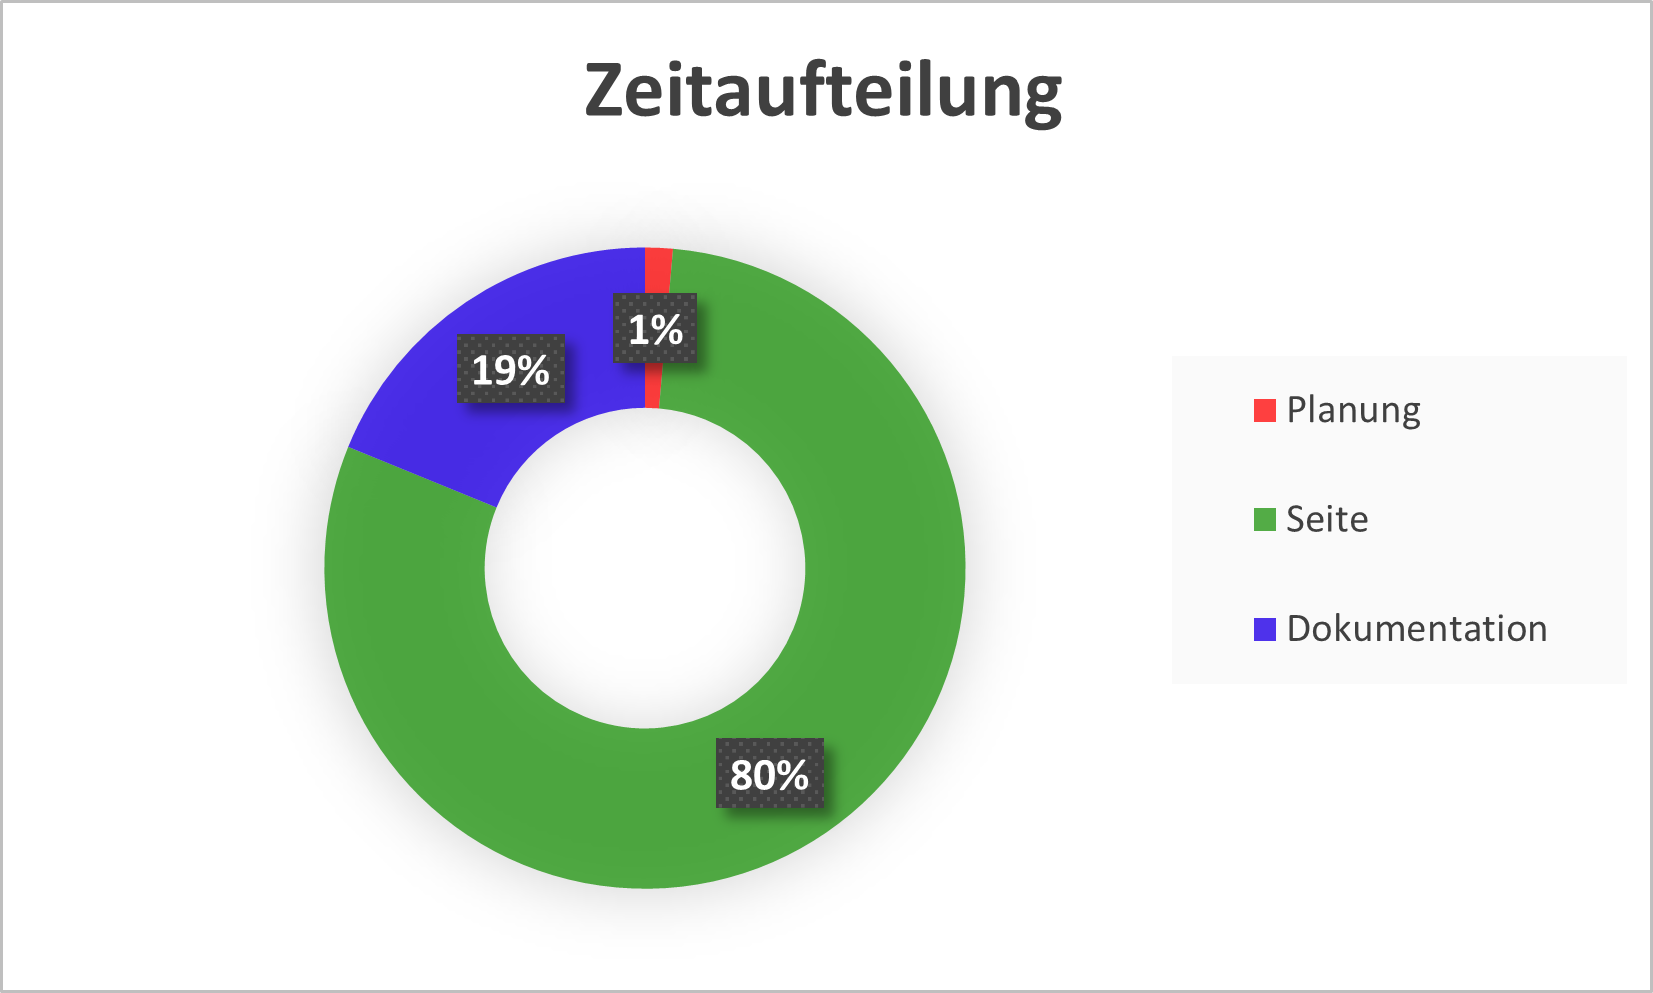
\includegraphics[width=1\textwidth]{images/Zeiten/Zeitaufteilung-Bertoni.png}
        \caption{Verteilung von Alexanders Arbeitsstunden}
    \end{center}
\end{figure}

\begin{figure}[H]
    \begin{center}
        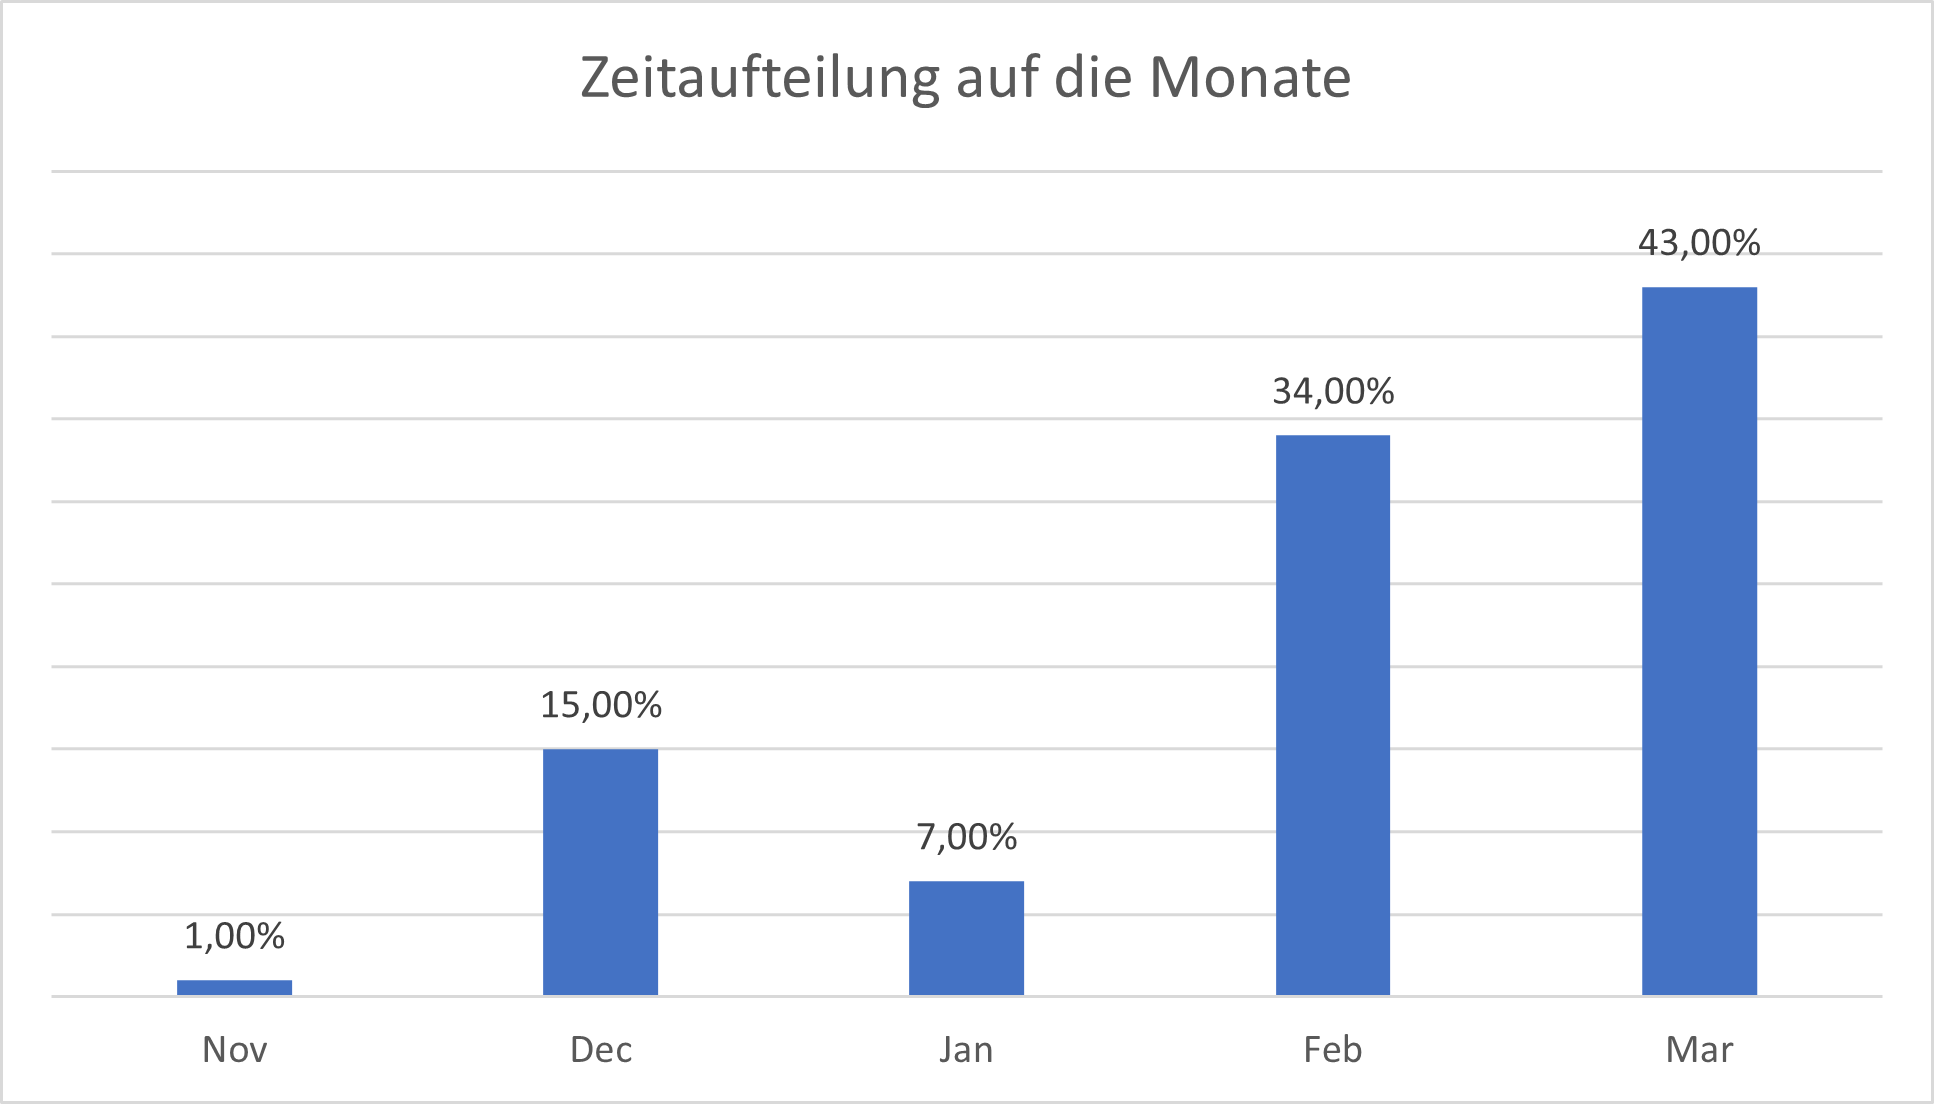
\includegraphics[width=1\textwidth]{images/Zeiten/Zeitaufteilung-auf-Monate-Bertoni.png}
        \caption{Alexanders Arbeitszeiten vom 29.01.2020 bis zum 24.03.2022}
    \end{center}
\end{figure}

\section*{Arbeitsprotokoll - Joshua Winkler}

\begin{table}[H]
    \begin{tabular}{lrr}
        \hline
        \textbf{Projekt} & \multicolumn{1}{l}{\textbf{Arbeitsaufwand}} & \multicolumn{1}{l}{\textbf{Prozentueller Anteil}} \\ \hline
        \fcolorbox{black}{Planung}{\rule{0pt}{4pt}\rule{4pt}{0pt}} Planung & 8:52:30 & 4.81\% \\
        \fcolorbox{black}{Backend}{\rule{0pt}{4pt}\rule{4pt}{0pt}} Backend & 77:07:14 & 41.82\% \\
        \fcolorbox{black}{ACP}{\rule{0pt}{4pt}\rule{4pt}{0pt}} ACP & 66:08:50 & 35.87\% \\
        \fcolorbox{black}{Dokumentation}{\rule{0pt}{4pt}\rule{4pt}{0pt}} Dokumentation & 32:16:37 & 17.50\% \\
        \hline
        \textbf{Summe} & \textbf{184:25:11} & \textbf{100.00\%} \\
        \hline
    \end{tabular}
\end{table}

\begin{figure}[H]
    \begin{center}
        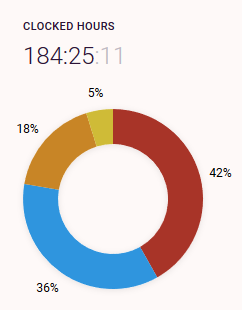
\includegraphics[width=0.30\textwidth]{images/Appendix/Josh/clockedHours.png}
        \caption{Verteilung von Joshuas Arbeitsstunden}
    \end{center}
\end{figure}

\begin{figure}[H]
    \begin{center}
        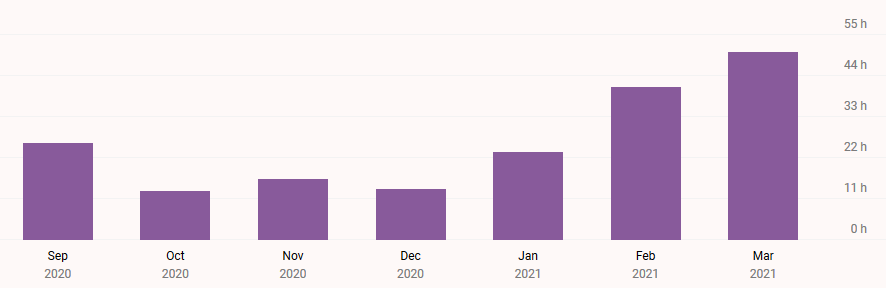
\includegraphics[width=1\textwidth]{images/Appendix/Josh/timeline.png}
        \caption{Joshuas Arbeitsverlauf vom 14.09.2020 bis zum 26.03.2021}
    \end{center}
\end{figure}
